\section{Implementacija}
\label{sec:impl}

Program koji automatizuje proces opisan u poglavlju \ref{sec:Drawing} je dostupan na GitHub-u: \url{https://github.com/ivan-ristovic/epicyclez}. Implementiran u \texttt{C\#}-u 7.3, trenutno dostupan samo za \texttt{Windows} operativni sistem \footnote{Sa izdanjem 3.0 .NET Core radnog okvira, program \'c{}e biti mogu\'c{}e pokrenuti na svim operativnim sistemima koji imaju instaliran .NET Core Runtime.}. Prikaz rada programa se mo\v{z}e videti na slici \ref{fig:impl}.

\begin{figure}
    \centering
    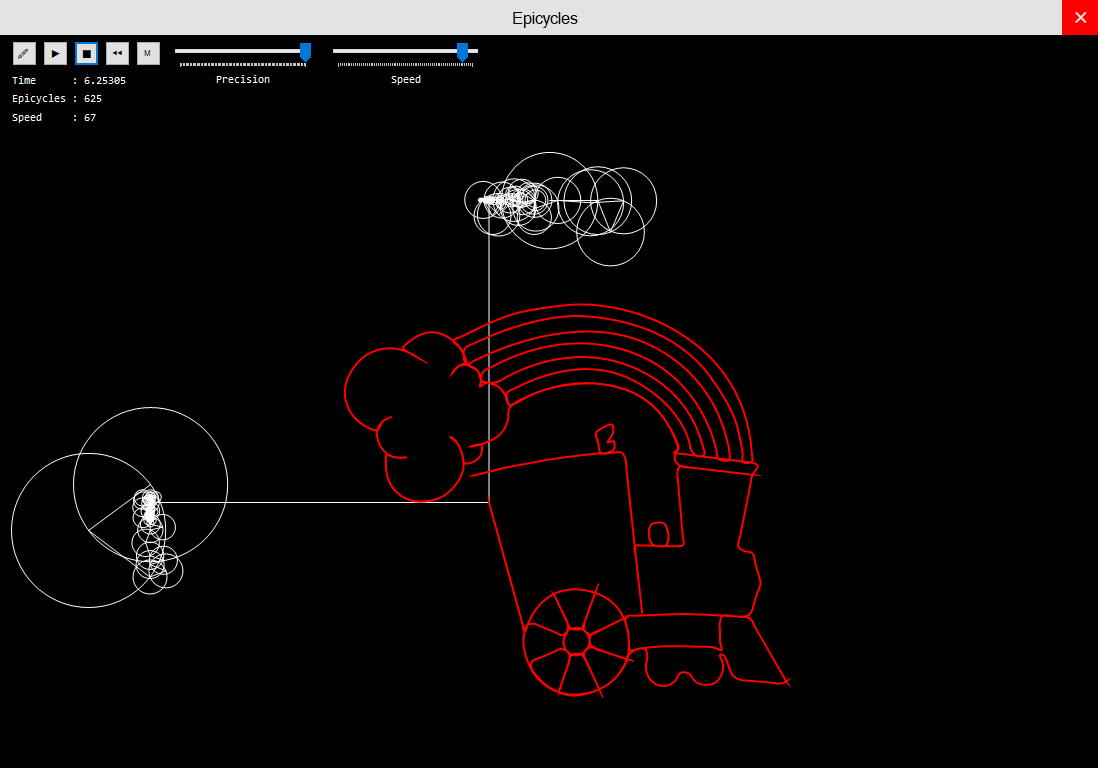
\includegraphics[scale=0.37]{images/impl1.PNG}
    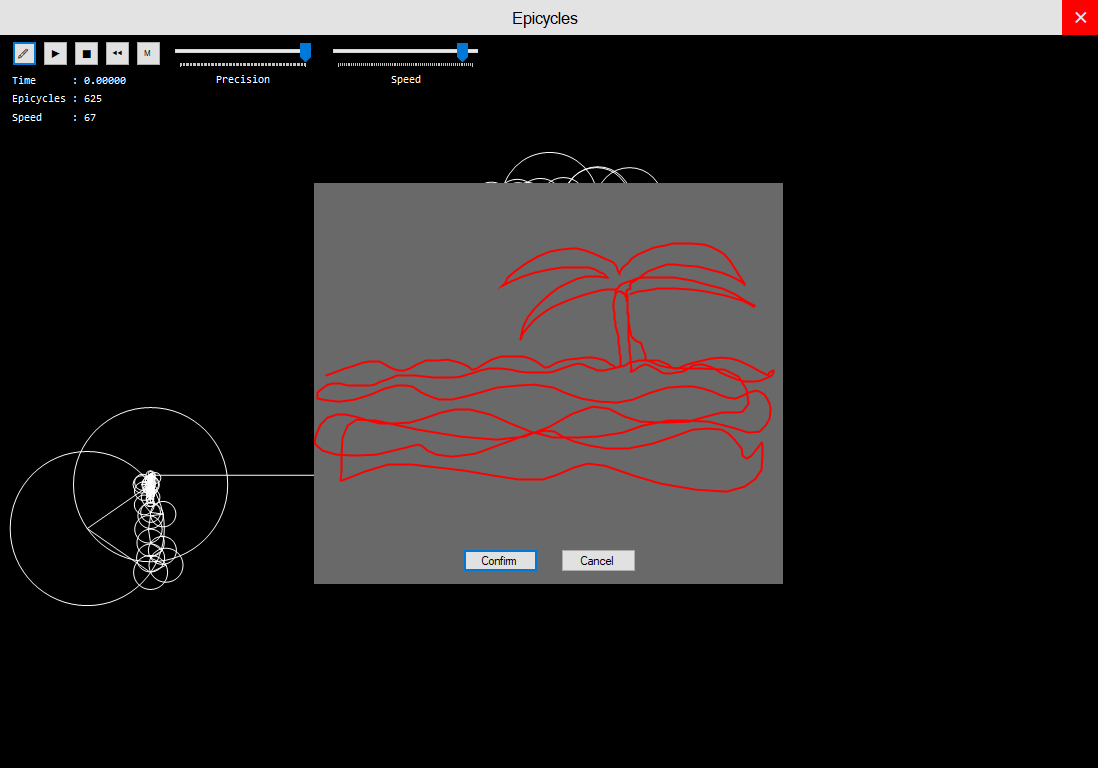
\includegraphics[scale=0.37]{images/impl2.PNG}
    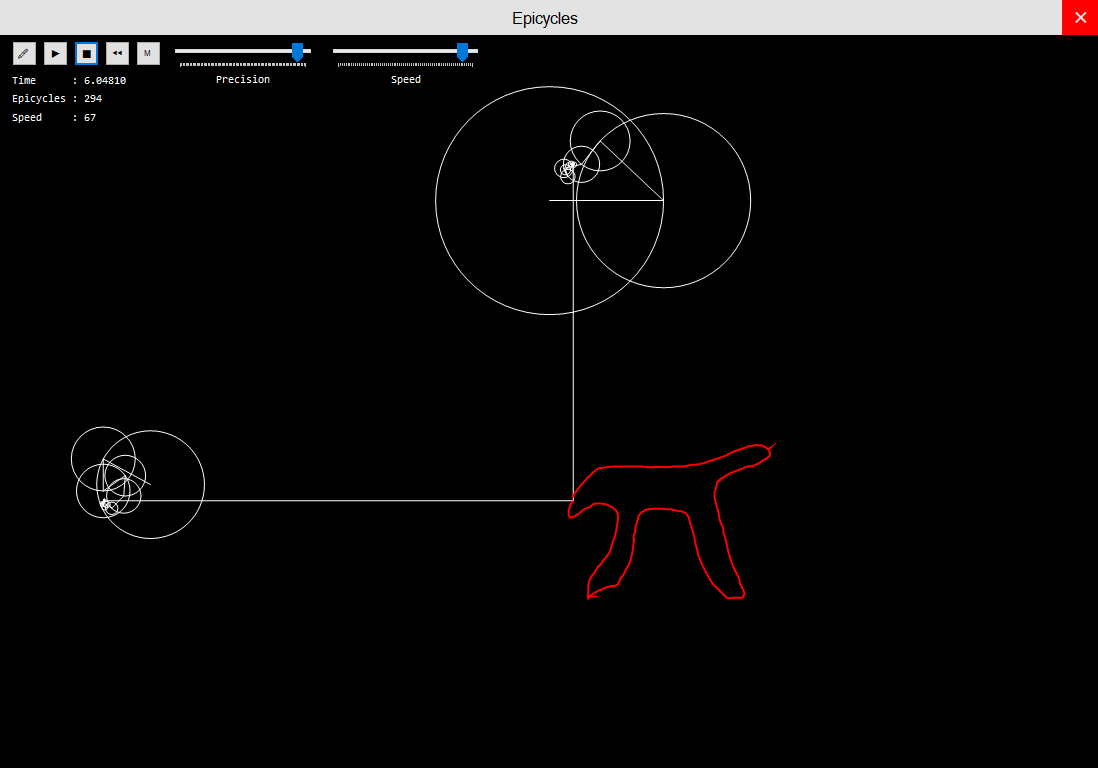
\includegraphics[scale=0.37]{images/impl3.PNG}
    \caption{Prikaz rada programa. Mogu\'c{}e je crtati proizvoljne ru\v{c}no iscrtane konture ili u\v{c}itati signal u \texttt{json} formatu.}
    \label{fig:impl}
\end{figure}

